\documentclass[russian,utf8,nocolumnxxxi,nocolumnxxxii]{eskdtext}
\usepackage[T1,T2A]{fontenc}
\usepackage[utf8]{inputenc}
\usepackage{graphicx}
\graphicspath{{pictures/}}
\usepackage{pgfplots}
\pgfplotsset{compat=1.9}
%\usepackage[english,russian]{babel}
\usepackage{amssymb,amsmath}
\usepackage{tikz}
\usepackage{siunitx}
\usepackage{nccmath}

\usepackage[american,cuteinductors,smartlabels]{circuitikz}
\usepackage[backend=biber]{biblatex}
\addbibresource{error_estimation_otchet.bib}
\usepackage[]{hyperref}
\hypersetup{colorlinks=true,}
\usepackage{textcomp}
\usepackage{float}
\newcommand{\No}{\textnumero}
\ESKDdepartment{Федеральное агентство по образованию}
\ESKDcompany{Санкт-Петербургский государственный электротехнический университет "ЛЭТИ"}
\ESKDtitle{Пояснительная записка к Курсовой работе}


\ESKDsignature{Вариант N23}
\ESKDauthor{Рахманов ~М.~А.}
\ESKDchecker{Прокшин~А.~Н.}
\ESKDdocName{по дисциплине "Информатика"}

\begin{document}
\maketitle


{\normalsize{\bf{Содержание}}
\\1. Цель и тема курсовой работы
\\2. Задание на курсовую работу
\\3. Введение
\\4. Исследование функции
\\5. Исследование кубического сплайна
\\6. Задача оптимального распределения неоднородных ресурсов
\\7. Список литературы
\newpage
\normalsize{\bf{Цель курсовой работы:}} уметь применять персональный компьютер и
математические пакеты прикладных программ в инженерной деятельности.
\par
\normalsize{\bf{Тема курсовой работы:}} решение математических задач с использованием
математического пакета "Scilab"или "Reduce-algebra".
\newpage
\begin{center}
 {\large\bf2. Задание на курсовую работу}
\end{center}
\normalsize1. Даны функции $f(x)=\sqrt{3}sin(x)+cos(x),g(x)=cos(2x+\frac{\pi}{3})-1$
\\а)Решить уравнение f(x)=g(x).
\\б)Исследовать функцию h(x)=f(x)-g(x) на промежутке $[0;\frac{5\pi}{6}]$
\\2. Найти коэффициенты кубического сплайна, интерполирующего данные, представленные в векторах:\\
$V_{x}=[0,1.25,2,2.625,4.25]$
$V_{y}=[4,3.925,4.675,4.8,4.956]$\\
Построить на графике функции f(x),полученную после нахождения коэффициентов кубического сплайна. \\
Представить графическое изображение результатов интерполяции исходных данных различными методами с использованием встроенных функций\\ splin(x,y,“natural”), splin(x,y,“clamped”), splin(x,y,“not\_a\_knot”), splin(x,y, “fast”), splin(x,y,“monotone”), interp(xx,x,y,d)\\
3. Решить задачу оптимального распределения неоднородных ресурсов.
Требуется решить следующую задачу оптимального распределения неоднородных ресурсов. Пусть в распоряжении завода железобетонных изделий (ЖБИ) имеется m видов сырья (песок, щебень, цемент) в объемах ${ a_i}$  .Требуется произвести продукцию { n} видов. Дана технологическая норма $c_ij$  требления отдельного i-го вида сырь для изготовления единицы продукции каждого j-го вида. Известна прибыль $\pi_j$  получаема от выпуска единицы продукции j-го вида. Требуется определить, какую продукцию и в каком количестве должен производить завод ЖБИ, чтобы получить максимальную прибыль.
\par
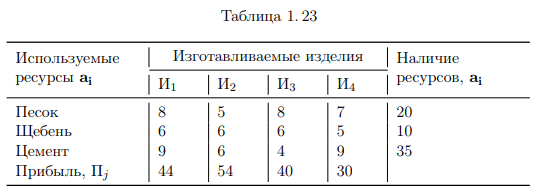
\includegraphics[scale=0.75]{2019-01-09_01-47-19}
\newpage
\begin{center} {\bf3. Введение} \end{center}
\par
\normalsize В современном мире технологие неудержимо летят вперед, с каждым годом электронно вычеслительная техника становиться мощьнее, компактнее и сложнее, а людям приходиться решать все более сложные задачи. С этим людям стали помогать математические пакеты и системы компьютерной алгебры, которые во много раз сокращают время на решение сложнейших задачь, с безчисленым количеством чисел, сейчас такие программы доступны каждому хоть и не все они бесплатные.
\newpage
\begin{center}{\bf4. Исследование функции} \end{center}
\par
\normalsize1. Даны функции:
\\$f(x)=\sqrt{3}sin(x)+cos(x)$\\ 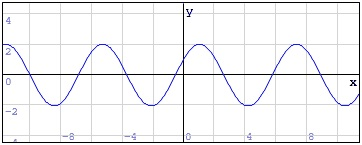
\includegraphics{f(x)}
\\$g(x)=cos(2x+\frac{\pi}{3})-1$\\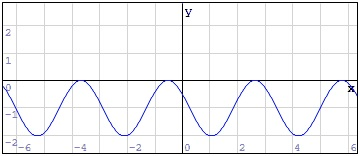
\includegraphics{g(x)}
\\а)Решить уравнение f(x)=g(x).
\\б)Исследовать функцию h(x)=f(x)-g(x) на промежутке $[0;\frac{5\pi}{6}]$\\
{\bfРешение уравнения.}
\\ f(x)=g(x)= f(x)-g(x)=0
\\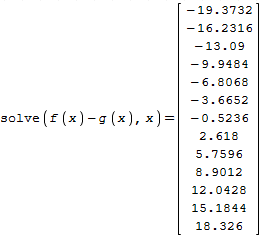
\includegraphics{2019-01-09_02-19-12}
\newpage

\par
\normalsize
Рассмотрим функцию h(x)=f(x)-g(x)
\\ h(x)=f(x)-g(x)
\\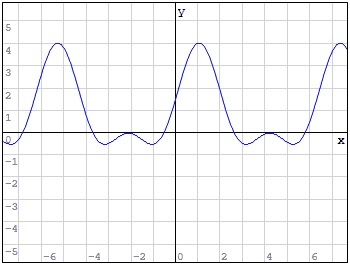
\includegraphics[scale=0.95]{h(x)=f(x)-g(x)}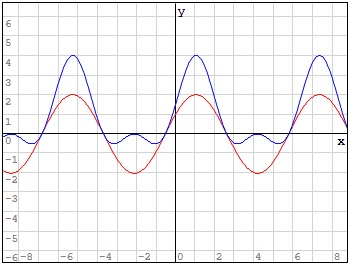
\includegraphics[scale=0.95]{f(x)-f(x)+f(x)}
\\Функция f(x)=g(x)= f(x)-g(x)=0 на промижутке $x=0$ до $x=\frac{5\pi}{6}$ \\
\begin{tikzpicture}

\begin{scope}[scale=2.7]

\draw[thin, ->] (0,0) -- (4,0) node[right] {$X$};
\draw[thin, ->] (0,0) -- (0,5) node[left] {$Y$};



\foreach \x\xtext in {0,2.618/\frac{5\pi}{6}} 
\draw (\x,0.1) -- (\x,-0.1) node[below] {$\xtext$};

\draw[domain=0:(5*3.14)/6, smooth, blue] plot ({\x},{(sqrt(3)*sin(\x r)+cos(\x r))-(cos(\x*2 r + pi/3 r)-1))});


\end{scope};

\end{tikzpicture}
\newpage
Найдем корни и пересечения с осями.
\\Jбласть определения функции задана и ровна от $x=0$ до $x=\frac{5\pi}{6}$
\\Так как функция h(x)является функцией обшего вида то и на области определения она также обладает общим видом если брать функцию h(x)полностью то она переодична  но так как область определения составляет (0:$\frac {5\pi}{6}$) функция не повторяется в области определения что означает у нее отсутствует периодичность.
\par
\normalsize
1.Найдем пересичение с осью Х:
\\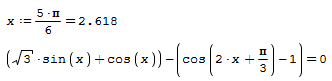
\includegraphics[scale=0.90]{2019-01-11_02-56-05}
\\2.Найдем пересичение с осью Y:
\\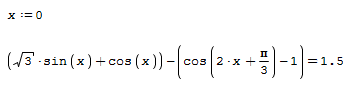
\includegraphics[scale=0.90]{2019-01-11_02-56-50}
\\3.Найдем экстремулу в пределах облости определения:
\\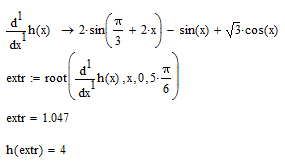
\includegraphics[scale=1]{2019-01-11_03-18-55}
\\4.Функция не имеет разрывов 
\\5.Так как функция являеться изначально синусоидальной асимптот не имеет
\\6.Имеет выпуклость (0;2618) 
\\7.Точек перегибов не имеет

\newpage
\begin{center}{\bf5. Исследование кубического сплайна.}\end{center}
\par
\normalsize Найти коэффициенты кубического сплайна, интерполирующего данные, представленные в векторах:\\
$V_{x}=[0,1.25,2,2.625,4.25]$
$V_{y}=[4,3.925,4.675,4.8,4.956]$\\
Построить на графике функции f(x),полученную после нахождения коэффициентов кубического сплайна. 
\\Оценить погрешность интерполяции в точке x=3.1. Вычеслить значение функции в точке x=2.1
\\Представить графическое изображение результатов интерполяции исходных данных различными методами с использованием встроенных функций\\ splin(x,y,“natural”), splin(x,y,“clamped”), splin(x,y,“not\_a\_knot”), splin(x,y, “fast”), splin(x,y,“monotone”), interp(xx,x,y,d)\\
\newpage
\begin{center}{\bf Нахождение коэффициентов кубического сплайна.}\\\end{center}
По заданию даны координаты 5 точек:
\\\includegraphics[scale=0.8]{2019-01-11_23-58-09}
\par
\normalsize
Найдем уравнение сплайна проходящего через пять точкек $(x_{1}, y_{1}),\\
(x_{2}, y_{2}), (x_{3}, y_{3}) и (x_{4}, y_{4})$. Для того чтобы потенциальная энергия изогнутой
металлической линейки(сплайна) принимала минимальное значение,
производная четвертого порядка должна быть равна нулю, значит мы
можем представить сплайн полиномом третьей степени на каждом отрезке
$[x_i, x_{i+1}]$
\\$$F_i(x) = A_{i0} + A_{i1}x + A_{i2}x^2 + A_{i3}x^3, где x \in [x_i, x_{i+1}]$$

\par
\normalsize По такому же принципу состовляем 8 уровнений, по два на каждый участок кривой.
\begin{center}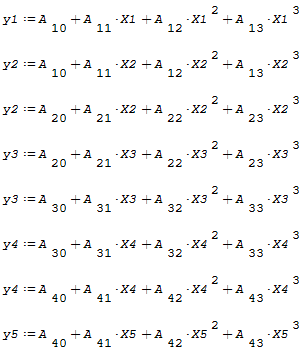
\includegraphics[scale=0.8]{2019-01-09_03-19-11}\end{center}
\par
\newpage
\normalsize
Для того что бы не было излома сплайна, добавляем три уровнения с производными певого порядка, по одному на каждое соединение.
\begin{center}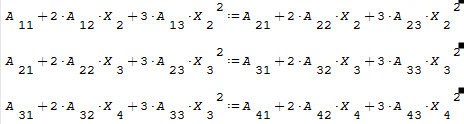
\includegraphics[scale=0.8]{2019-01-09_03-26-45}\end{center}
\par
\normalsize
Для получения одинакового изгиба с каждой стороны стыков, добавляем три уровнения с производными второго порядка.
\begin{center}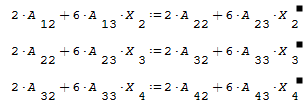
\includegraphics[scale=0.8]{2019-01-09_03-31-08}\end{center}
\par
\normalsize
Добавим уровнения отвечающие за положение концов сплайна, в нашем случае они оставлены свободно.
\begin{center}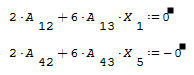
\includegraphics[scale=0.8]{2019-01-09_03-34-49}\end{center}
\newpage
\par
\normalsize
Таким образов были найдены 16 уровнений из которых можно составить матрицу размерностью 16х16. С ее помощью, решая матричное уравнение, находим коофиценты кубического сплайна.
\begin{center}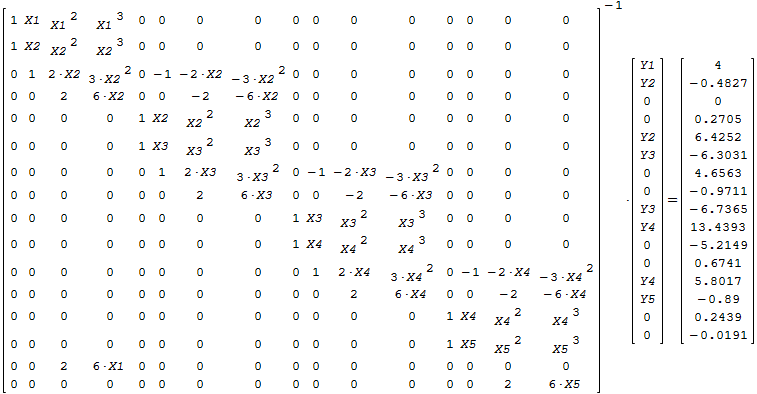
\includegraphics[scale=0.6]{2019-01-09_03-36-31}\end{center}
\par
\normalsize
Получаем окончательное уровнение сплайна.
\begin{center}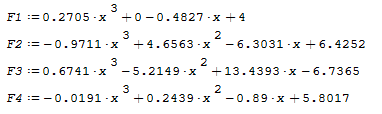
\includegraphics[scale=0.75]{2019-01-09_03-42-54}\end{center}
\newpage
\begin{center}{\bf построение кубического сплайна.}\\\end{center}
\begin{tikzpicture}

\begin{scope}[scale=2]


\draw[thin, ->] (0,0) -- (6,0) node[right] {$X$};
\draw[thin, ->] (0,0) -- (0,6) node[left] {$Y$};

\foreach \x\xtext in {,2,1,3,4,5} 
\draw (\x,0.1) -- (\x,-0.1) node[below] {$\xtext$};
\foreach \y\ytext in {2,1,3,4,5} 
\draw (0.1,\y) -- (-0.1,\y) node[left] {$\ytext$};


\draw[domain=0:1.25, smooth, blue] plot ({\x},{(0.2705*(\x)*(\x)*(\x))+0-(0.4827*(\x))+4});
\draw[domain=1.25:2, smooth, red] plot ({\x},{(-0.9711*(\x)*(\x)*(\x))+(4.6563*(\x)*(\x))-(6.3031*(\x))+6.4252});
\draw[domain=2:2.625, smooth,green] plot ({\x},{(0.6741*(\x)*(\x)*(\x))-(5.2149*(\x)*(\x))+(13.4393*(\x))-6.7365});
\draw[domain=2.625:4.25, smooth, violet] plot ({\x},{(-0.0191*(\x)*(\x)*(\x))+(0.2439*(\x)*(\x))-(0.89*(\x))+5.8017});



\draw (0,4) circle (0.8pt);
\draw (1.25,3.925) circle (0.8pt);
\draw (2,4.675) circle (0.8pt);
\draw (2.625,4.8) circle (0.8pt);
\draw (4.25,4.956) circle (0.8pt);
\draw (2.1,4.7312) circle (0.8pt);
\draw[red] (3.1,4.6061) circle (0.8pt) node[below]{Lagr};
\draw (3.1,4.8176) circle (0.8pt);

\draw[thin,dashed] (1.25,3.925) -- (1.25,0);

\draw[thin,dashed] (2,4.675)  -- (2,0) ;

\draw[thin,dashed]  (2.625,4.8) --  (2.625,0);

\draw[thin,dashed] (4.25,4.956) -- (4.25,0);




\end{scope};



\end{tikzpicture}
\\Найдем значение в точке 2.1 подставим в полином данного промижутка x=2.1
\\\includegraphics[scale=0.7]{2019-01-12_00-09-00}
\\\includegraphics[scale=0.7]{2019-01-12_00-10-00}
\newpage
\begin{center}

{\bf Оценка погрешности при интерполяции полиномом
Лагранжа}

\end{center}

Лагранж, Жозеф Луи предложил для интерполяции использовать многочлен
вида:
$$L(x)=\sum\limits_{i=1}^ny_il_i(x)$$
\\где базисные полиномы определяются по формуле:
$$l_i(x)=\prod\limits_{j = 0 j \neq i}^n \frac{x-x_j}{x_i-x_j}=\frac{x-x_0}{x_i-x_0}\ldots \frac{x-x_{i-1}}{x_i-x_{i-1}}*\frac{x-x_{i+1}}{x_i-x_{i+1}}\ldots \frac{x-x_{n}}{x_i-x_{n}}$$


Используя исходные данные подставим их в формулу:
\begin{center}
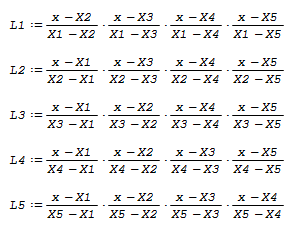
\includegraphics[scale=0.7]{2019-01-11_01-38-55}
\end{center}

\begin{center}
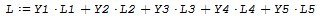
\includegraphics[scale=0.7]{2019-01-11_01-39-59}
\end{center}
Подставим x=3.1 и получим значение в этой точке равное 4.6061
\\используя полином данного участка из прошлой главы найдем значение в этой же точке, оно равно 4.8176

\begin{center}
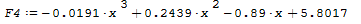
\includegraphics[scale=0.7]{2019-01-11_01-41-56}
\end{center}
Вычтя из одного другое получим что погрешность в конкретно взятой точке относительно полинома Лагранжа состовляет 0.2115
\par
\normalsize

\newpage

\begin{center}

{\bf Оценка погрешности интерполяции Эрмитовыми
кубическими сплайнами}

\end{center}
Для того что бы найти погрешность данным способом нам нужно получить четвертую производную функции:
После этого подставляем в формулу получившуюся производную, и вычесляем h подставляем заданую точку 3.1 и ближайшую к ней то есть 2.625
\\\includegraphics[scale=0.7]{2019-01-12_00-01-19}

\newpage
{\bf6. Задача оптимального распределения неоднородных ресурсов.}\\
Требуется решить следующую задачу оптимального распределения неоднородных ресурсов. Пусть в распоряжении завода железобетонных изделий (ЖБИ) имеется m видов сырья (песок, щебень, цемент) в объемах $ a_i$  .Требуется произвести продукцию n видов. Дана технологическая норма $c_ij$  требления отдельного i-го вида сырь для изготовления единицы продукции каждого j-го вида. Известна прибыль $П_j$  получаема от выпуска единицы продукции j-го вида. Требуется определить, какую продукцию и в каком количестве должен производить завод ЖБИ, чтобы получить максимальную прибыль.\\
Исходные данные:\\

\begin{center}
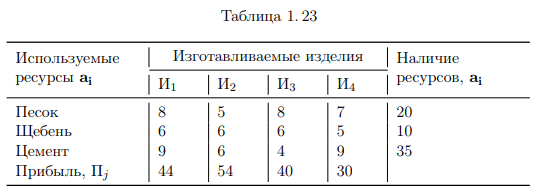
\includegraphics[scale=0.7]{2019-01-09_01-47-19}
\end{center}
Так как данная задача является целочисленной задачей линейного программирования, стандартная функция мат. пакета «SciLab» для решения задач линейного программирования karmarkar не даст верного решения, так как не учитывает целочисленное ограничение
\newpage
\par
\normalsize
Для решения задачи воспользуемся пакетом lpsolve:

[x,f] =  $lp\_solve(F,a,B,e,vlb,[],xint), где:$

a – матрица значений технологической норм

B – вектор ограничений на объем используемого сырья

F – вектор значений целевой функции - прибыли

e – вектор, определяющий оператор отношения для ограничений $(\leq  =  \geq)$

vlb – вектор, задающий нижнюю границу переменных

xint – вектор, задающий целочисленное ограничение на переменные


a = [8,5,8,7;6,6,6,5;9,6,4,9];

B = [20;10;35];

F = [44,54,40,30];

e = [-1,-1,-1];

vlb = [0,0,0];

xint = [1,2,3,4];

[x,f] =$lp\_solve(F,a,B,e,vlb,[],xint)$

x = [0;0;0;2]

f = 60.

Таким образом, искомым целочисленным решением доставляющим максимум целевой функции является вектор [0;0;0;2], а значением целевой функции, отвечающему этому вектору = 60. Следовательно что бы получить максимальную прибыль равной 60 условных единиц, заводу нужно произвести изделие И$_4$ в размере двух штук.

\newpage
\begin{center} {\bf6. Вывод} \end{center}
Были изучены возможности разных математических программ, получино умение выбирать для работы программу наиболее эфективную для решения поставленной задачи. Были решены задачи по изучению функции, построению сплайна и нахождению его погрешности двумя способами и обнаружено что оценка погрешности Эрмитовыми кубическими сплайнами дает более точные показания чем метадом Лагранжа, решению задачи с целочисленным програмированием.



\newpage
{\bf8. Список литературы}
\\1. Ю.С. Завьялов. Методы сплайн-функций. М.Наука, 1980.
\\2. Introduction in SciLab
\\3. https://ru.wikipedia.org/wiki/Интерполяционный\_многочлен\_Лагранжа
\\4.http://lpsolve.sourceforge.net/5.1/Scilab.htm
\\5.smath studio user’s manual
































\end{document}